\chapter{Results}
\begin{comment}


\end{comment}

\section{Results from the Lenard-Jones Potential with direct Summation}
\begin{comment}

\end{comment}

% Simulation Snapshots
\begin{figure}[!h]
	\begin{center}
		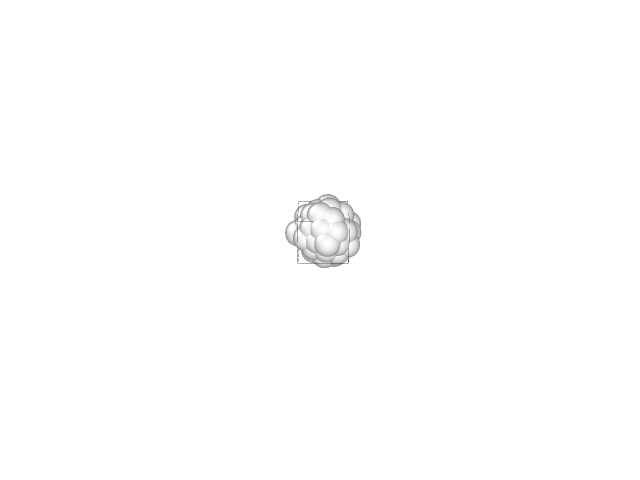
\includegraphics[scale= 1]{Figure/1Image.png}
	\end{center}
	\caption[Simulation]{Simulation }
	\label{SimulationSnapshot1}
\end{figure}

\begin{figure}[!h]
	\begin{center}
		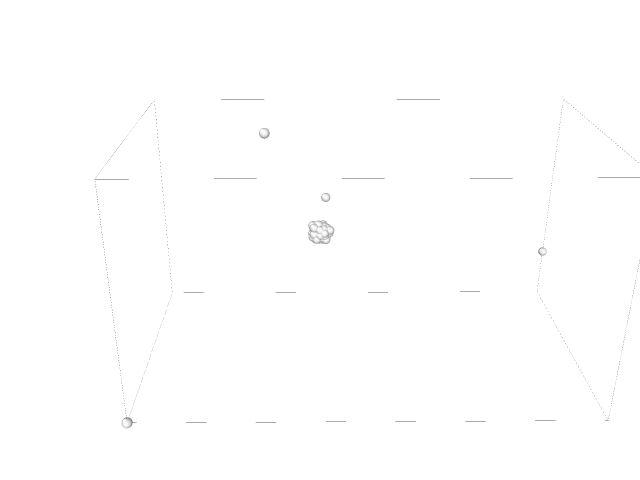
\includegraphics[scale= 1]{Figure/3Image.png}
	\end{center}
	\caption[Simulation]{Simulation }
	\label{SimulationSnapshot2}
\end{figure}

% Plot of the total energy as a function of time

%TODO make Nicer or plot into on lol
\begin{figure}[!h]
	\begin{center}
		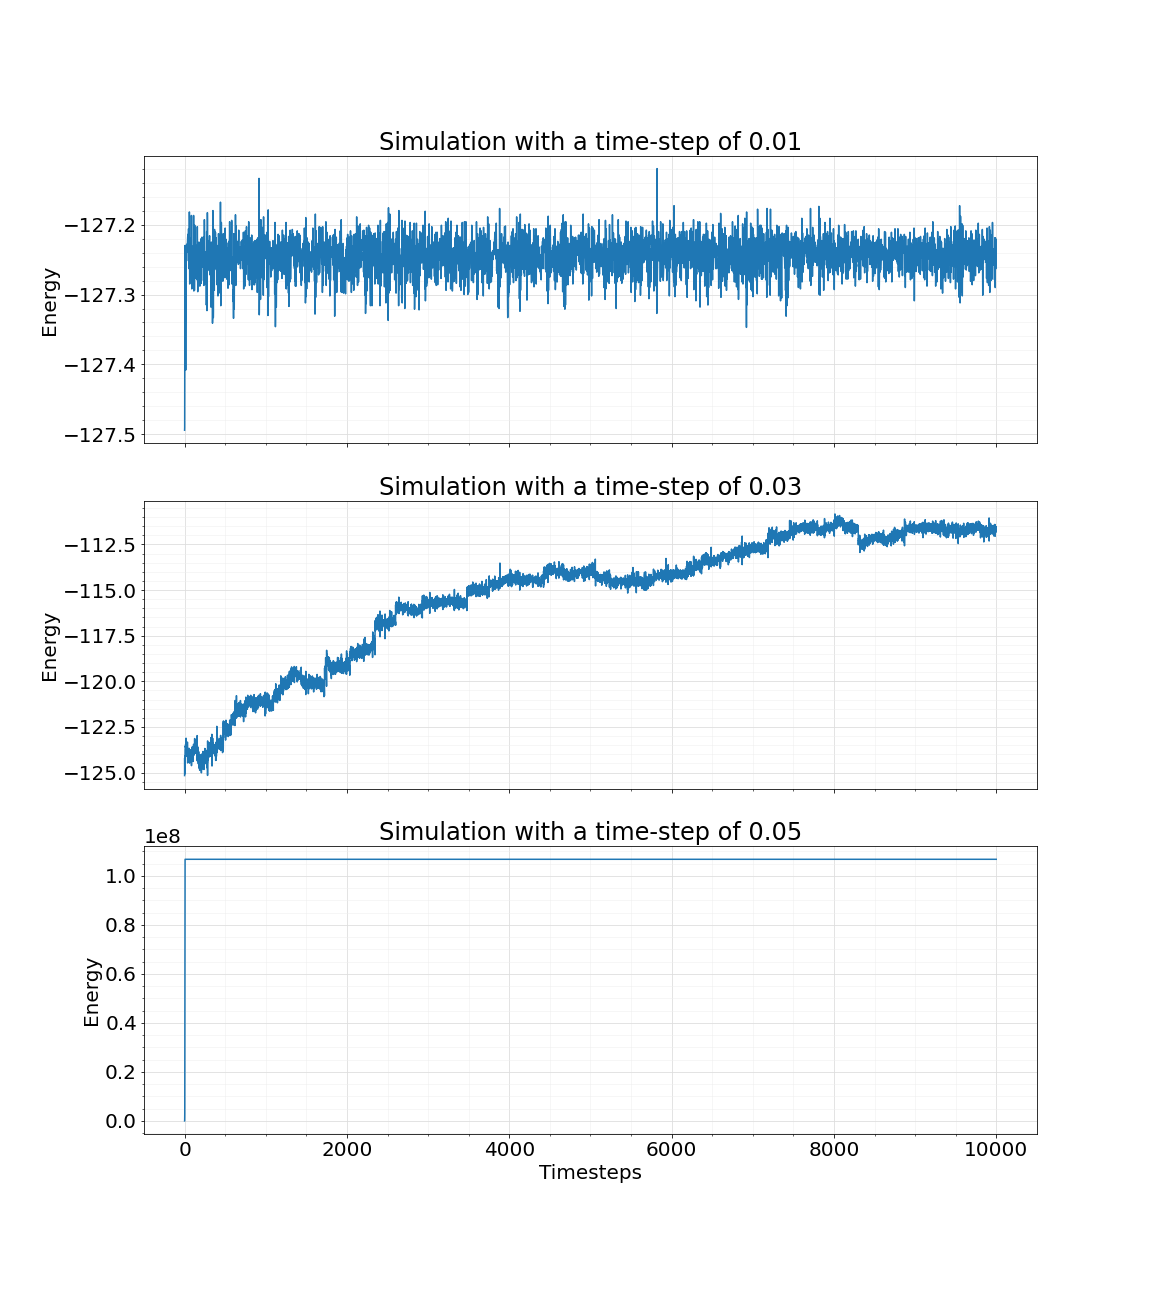
\includegraphics[scale= 1]{/home/cm/CLionProjects/MDCode/AData//totalEnergyDrift.png}
	\end{center}
	\caption[Simulation]{Simulation }
	\label{SimWithTimestep}
\end{figure}

\section{Result from the Simulation with the Berendsen Thermostat}
\begin{comment}

\end{comment}


\begin{figure}[!h]
	\begin{center}
		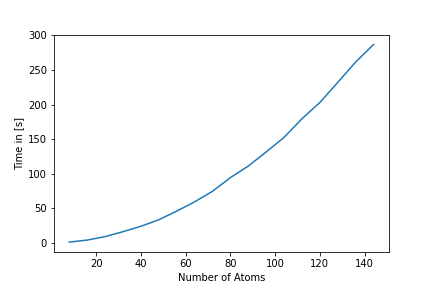
\includegraphics[scale=1]{Figure/plotAtomTimes.png}
	\end{center}
	\caption[Simulation-time with the Berendsen Thermostat from 8 to 192 Atoms]{Simulation-time with the Berendsen Thermostat from 8 to 192 Atoms }
	\label{PlotSimulationTimeBerendsenThermostat}
\end{figure}


\section{Results from the Simulation with the Neighborhood-List}
\begin{comment}

\end{comment}

\begin{figure}[!h]
	\begin{center}
		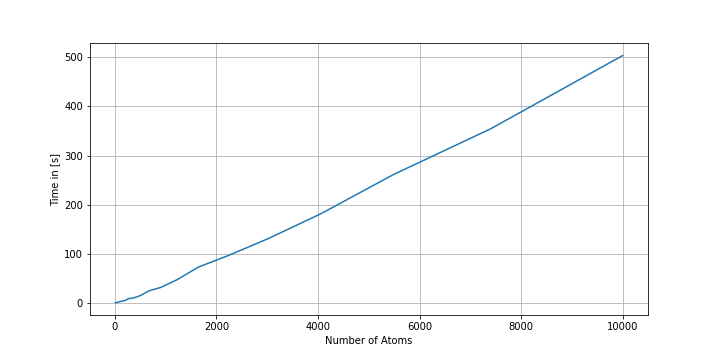
\includegraphics[scale=1.25]{Figure/plotAtomTimesMoreData.png}
	\end{center}
	\caption[Simulation-time with the Neighbor-list]{Simulation-time with the Neighbor list}
	\label{PlotSimulationTimesCutoffNew}
\end{figure}

\section{Results from the Simulation with the Gupta-Potential}
\begin{comment}

\end{comment}

\begin{figure}[!h] 
	\begin{center} 
		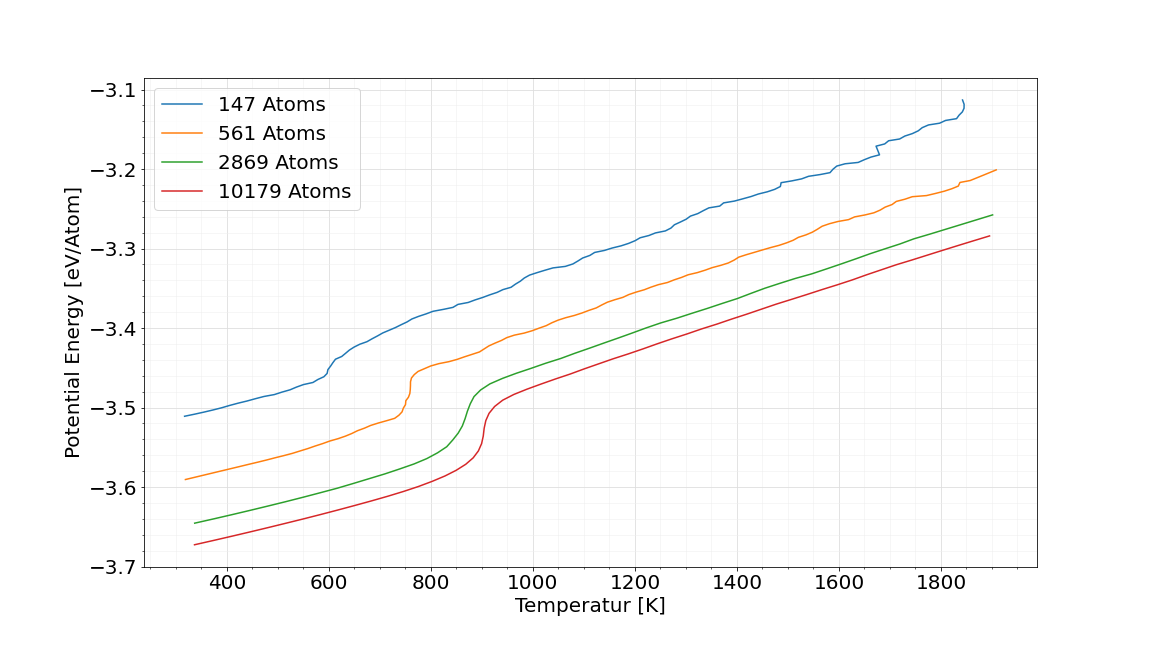
\includegraphics[scale=1.15]{/home/cm/CLionProjects/MDCode/AData/Clusters/temperaturPotentialEnergyCurveMoreInOne.png} 
	\end{center} 
	\caption[Gold Cluster Simulation]{Gold Cluster Simulation} 
	\label{GoldClusterSimulationTemperaturEnergy4In1} 
\end{figure} 

\begin{figure}[!h] 
	\begin{center} 
		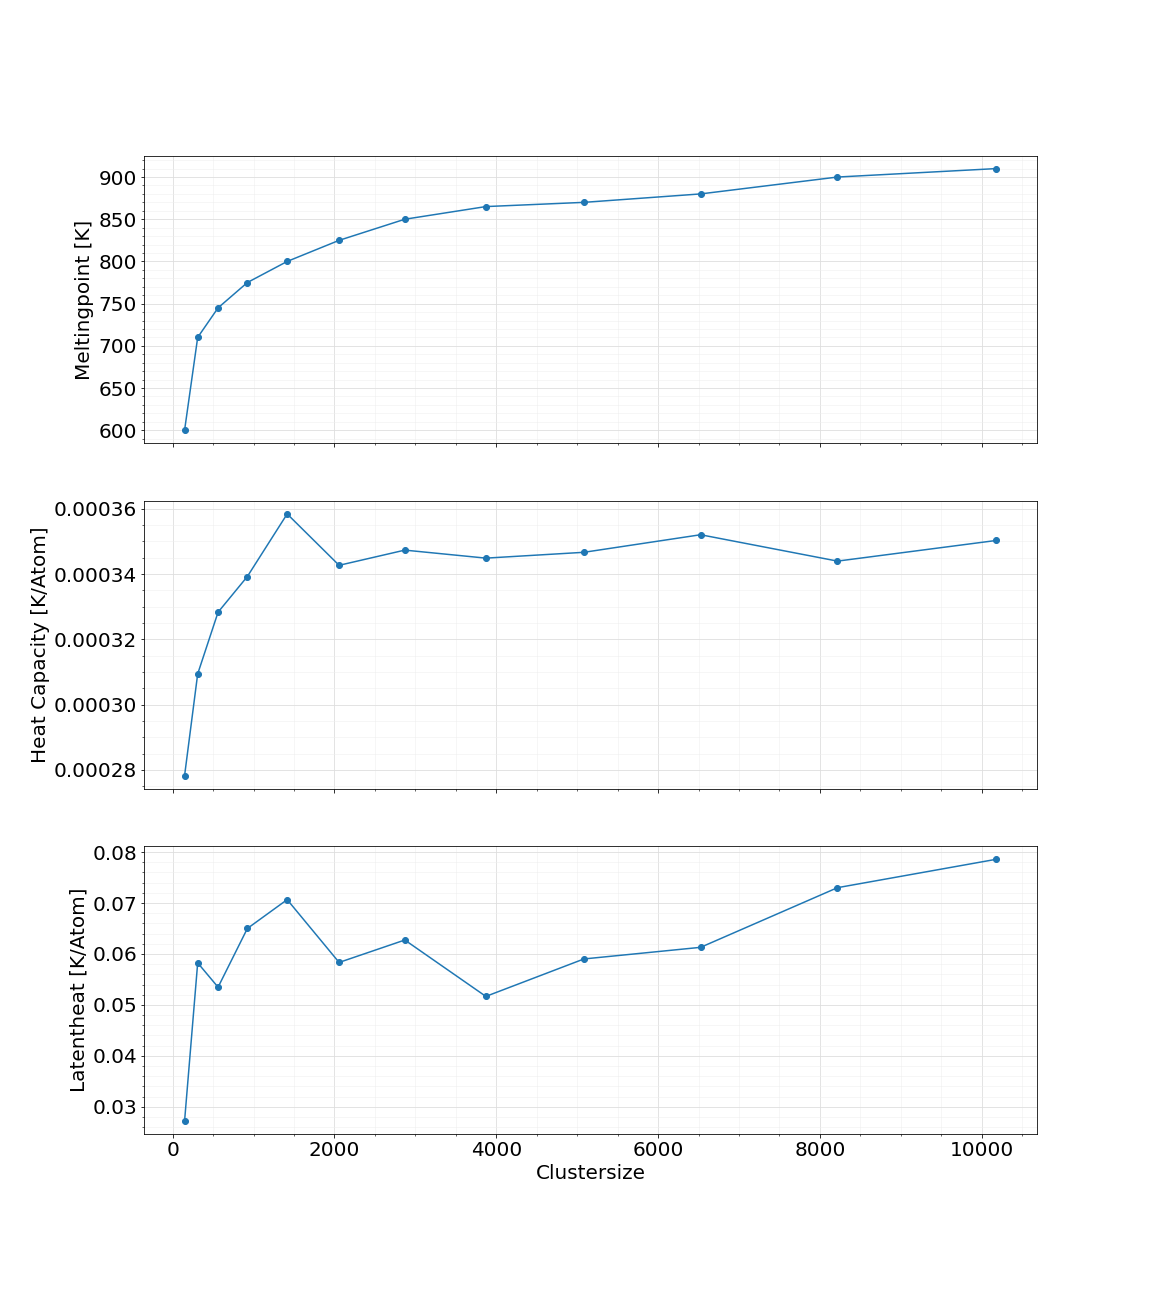
\includegraphics[scale=1.15]{/home/cm/CLionProjects/MDCode/AData/Clusters/VsClusterSizeAll.png} 
	\end{center} 
	\caption[Melting Point, Heat Capacity and Latent Heat vs Clustersize]{Melting Point, Heat Capacity and Latent Heat vs Clustersize} 
	\label{GoldClusterSimulationVsClustersize} 
\end{figure} 
